%%%%%%%%%%%%%%%%%%%%%%%%%%%%%%%%%%%%%%%%%%%%%%%%%%%%%%%%%%%%%%%%%%%%%%%%
% Escuela Politécnica Superior de la Universidad de Alicante
% Realizado por: Jose Manuel Requena Plens
% Contacto: info@jmrplens.com / Telegram:@jmrplens
%%%%%%%%%%%%%%%%%%%%%%%%%%%%%%%%%%%%%%%%%%%%%%%%%%%%%%%%%%%%%%%%%%%%%%%%

\definecolor{mycolor1}{rgb}{1.00000,0.00000,1.00000}%
%
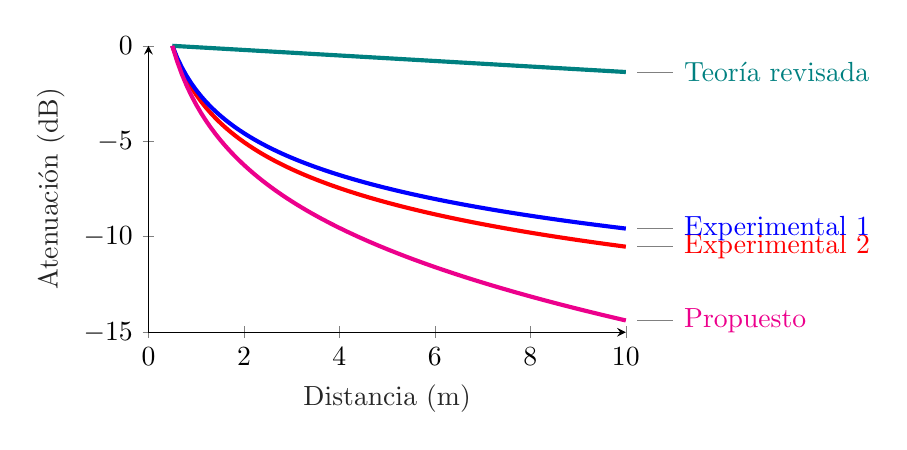
\begin{tikzpicture}

\begin{axis}[%
width=0.5\textwidth,
height=0.3\textwidth,
at={(0\textwidth,0\textwidth)},
scale only axis,
xmin=0,
xmax=10,
xlabel style={font=\color{white!15!black}},
xlabel={Distancia (m)},
ymin=-15,
ymax=0,
clip=false,
axis y line=left,
axis x line=bottom,
ylabel style={font=\color{white!15!black}},
ylabel={Atenuación (dB)},
axis background/.style={fill=white},
legend style={legend cell align=left, align=left, draw=white!15!black}
]
\addplot [color=red, line width=1.5pt]
  table[row sep=crcr]{%
0.5	0\\
0.6	-0.681268180014783\\
0.699999999999999	-1.25295926094489\\
0.800000000000001	-1.74500857405552\\
0.9	-2.1765973186647\\
1	-2.56074716972222\\
1.1	-2.90669889317459\\
1.2	-3.22124454315912\\
1.3	-3.50952085170319\\
1.4	-3.77550565273192\\
1.5	-4.02234137529044\\
1.6	-4.25255314804272\\
1.7	-4.46820017046615\\
1.8	-4.67098342349328\\
1.9	-4.86232399630538\\
2	-5.0434211434293\\
2.1	-5.21529605184143\\
2.2	-5.3788253372246\\
2.3	-5.53476702948237\\
2.4	-5.68378097985607\\
2.5	-5.8264450661754\\
2.6	-5.96326819238567\\
2.7	-6.09470081362625\\
2.8	-6.22114353077266\\
2.9	-6.34295416389409\\
3	-6.46045361629108\\
3.1	-6.57393076878918\\
3.2	-6.68364659036163\\
3.3	-6.78983761082107\\
3.4	-6.89271887067432\\
3.6	-7.08931957790021\\
3.8	-7.27482647442305\\
4	-7.45040225136549\\
4.2	-7.61703696130228\\
4.4	-7.77558049326828\\
4.6	-7.926767766015\\
4.8	-8.07123851294634\\
5	-8.20955299329626\\
5.2	-8.34220459532082\\
5.4	-8.46963004048317\\
5.6	-8.59221771596161\\
5.8	-8.71031453244824\\
6	-8.82423160940138\\
6.2	-8.93424902011984\\
6.4	-9.04061977703894\\
6.6	-9.14357319854545\\
6.9	-9.29204679768539\\
7.2	-9.43392442652032\\
7.5	-9.56975628814219\\
7.8	-9.70002691493798\\
8.1	-9.82516518961904\\
8.4	-9.94555252816818\\
8.7	-10.0615296145471\\
9	-10.1734019839036\\
9.3	-10.2814446824765\\
9.6	-10.3859061813585\\
10	-10.520003668456\\
}node [pos=1,pin=0:Experimental 2] {};

\addplot [color=blue, line width=1.5pt]
  table[row sep=crcr]{%
0.5	0\\
0.6	-0.616533326451801\\
0.699999999999999	-1.13423697060247\\
0.800000000000001	-1.58006665097912\\
0.9	-1.97130424956818\\
1	-2.31968785692216\\
1.1	-2.63355099833748\\
1.2	-2.91902130075722\\
1.3	-3.18073464726344\\
1.4	-3.42228218645896\\
1.5	-3.64650172146513\\
1.6	-3.85567422909482\\
1.7	-4.05166028861399\\
1.8	-4.23599718530805\\
1.9	-4.40996954116169\\
2	-4.57466167952575\\
2.1	-4.7309971094778\\
2.2	-4.87976875057399\\
2.3	-5.02166238498386\\
2.4	-5.1572750784906\\
2.5	-5.28712981115534\\
2.6	-5.41168721572554\\
2.7	-5.53135508318451\\
2.8	-5.64649612597388\\
2.9	-5.75743436821334\\
3	-5.86446044408093\\
3.1	-5.96783602060469\\
3.2	-6.06779751277566\\
3.3	-6.1645592225146\\
3.5	-6.34924554769489\\
3.7	-6.52325926309992\\
3.9	-6.68774631572047\\
4.1	-6.84367844680145\\
4.3	-6.99188671395386\\
4.5	-7.13308733082738\\
4.7	-7.2679018427927\\
4.9	-7.39687306465733\\
5.1	-7.52047780466582\\
5.3	-7.63913712157813\\
5.5	-7.75322466682555\\
5.7	-7.8630735249092\\
5.9	-7.96898186487812\\
6.1	-8.07121764229286\\
6.3	-8.17002253670066\\
6.6	-8.31226984728707\\
6.9	-8.44794078386757\\
7.2	-8.5776062281053\\
7.5	-8.70176622494593\\
7.8	-8.820861206242\\
8.1	-8.93528107943976\\
8.4	-9.04537265034821\\
8.7	-9.15144573311768\\
9	-9.25377821626172\\
9.4	-9.38483170886062\\
9.8	-9.51020492591051\\
10	-9.57090849682801\\
}node [pos=1,pin=0:Experimental 1] {};

\addplot [color=teal, line width=1.5pt]
  table[row sep=crcr]{%
0.5	0\\
10	-1.37246756153321\\
}node [pos=1,pin=0:Teoría revisada] {};

\addplot [color=magenta, line width=1.5pt]
  table[row sep=crcr]{%
0.5	0\\
0.6	-0.80625948743976\\
0.699999999999999	-1.49017441070941\\
0.800000000000001	-2.08454090744978\\
0.9	-2.6105131588871\\
1	-3.08253509145736\\
1.1	-3.51090897000311\\
1.2	-3.90324160586061\\
1.3	-4.26530969541624\\
1.4	-4.60160355609378\\
1.5	-4.9156828168317\\
1.6	-5.21041707979765\\
1.7	-5.48815349398464\\
1.8	-5.75083635819848\\
1.9	-6.00009434365721\\
2	-6.23730531773224\\
2.1	-6.46364533539513\\
2.2	-6.6801262232415\\
2.3	-6.88762480215888\\
2.4	-7.08690588606252\\
2.5	-7.27864058263035\\
2.6	-7.46342100258165\\
2.7	-7.64177219142685\\
2.8	-7.81416189022269\\
2.9	-7.98100858275356\\
3	-8.14268817792413\\
3.1	-8.29953959603374\\
3.2	-8.45186946785358\\
3.3	-8.5999561103969\\
3.4	-8.74405290900408\\
3.6	-9.02118280018142\\
3.8	-9.28488781260367\\
4	-9.53654581364221\\
4.2	-9.77733285826861\\
4.4	-10.0082607730785\\
4.6	-10.2302063789594\\
4.8	-10.4439344898265\\
5	-10.6501162133578\\
5.2	-10.8493436602727\\
5.4	-11.0421418760814\\
5.6	-11.2289786018407\\
5.8	-11.4102723213351\\
6	-11.5863989434692\\
6.2	-11.7576973885423\\
6.4	-11.9244742873256\\
6.6	-12.0870079568325\\
6.8	-12.2455517824032\\
7.1	-12.4763872234221\\
7.4	-12.6994620144316\\
7.7	-12.9153931497372\\
8	-13.1247268488223\\
8.3	-13.3279489835541\\
8.6	-13.5254936531196\\
8.9	-13.7177502880236\\
9.2	-13.9050695759205\\
9.5	-14.087768436244\\
9.8	-14.2661342211709\\
10	-14.382767518173\\
}node [pos=1,pin=0:Propuesto] {};


\end{axis}
\end{tikzpicture}%